\vspace{1cm}
\section{Análise de Desempenho da Aplicação}

Com o fim de elaborar uma análise de desempenho da aplicação \textbf{UmCarroJá}, utilizou-se a solução \textit{\textbf{Running Average Power Limit - RAPL}}.

\begin{figure}[H]
    \hbox{\hspace{-8em} 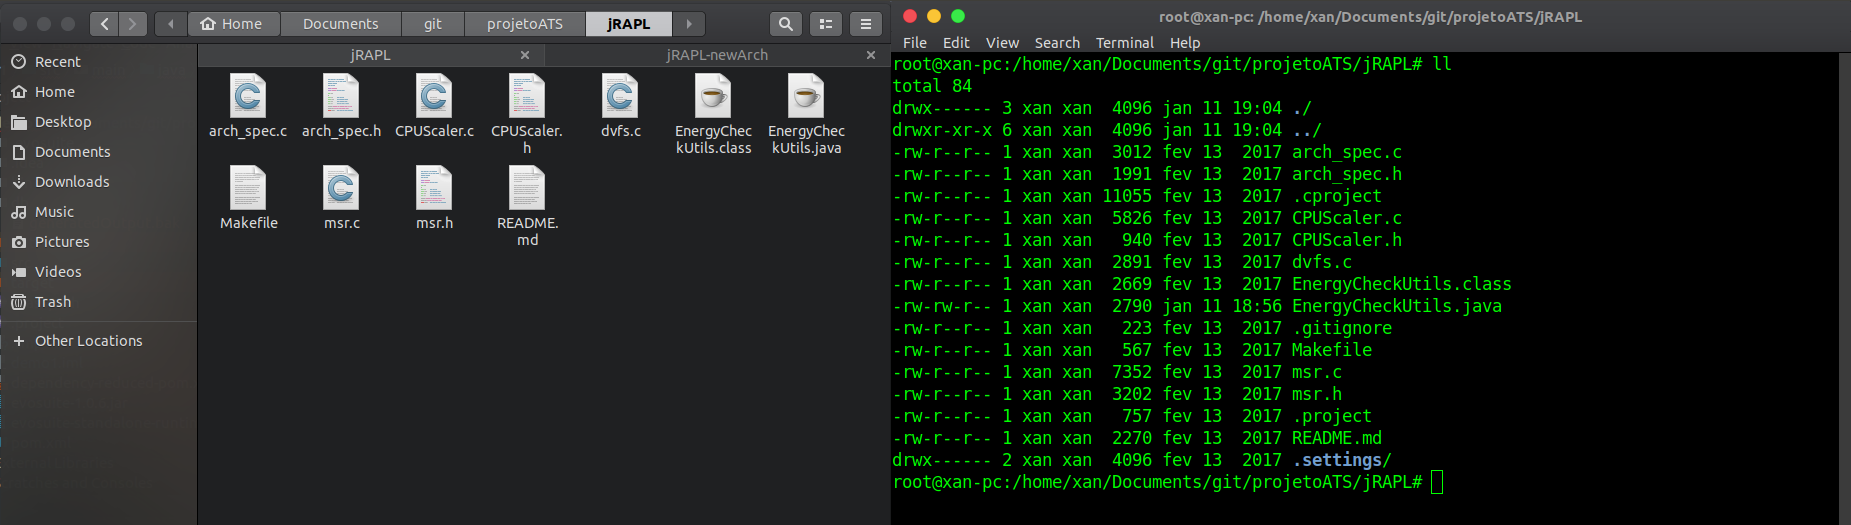
\includegraphics[width=1.5\textwidth]{images/rapl_inicial.png}}
    \label{fig47}
    \caption{Pasta inicial do jRAPL}
\end{figure}

\par Antes de se poder correr o \textit{RAPL} é necessário correr o comando \textit{make} com o intuito de compilar os ficheiros.\newline

\begin{figure}[H]
    \centering
    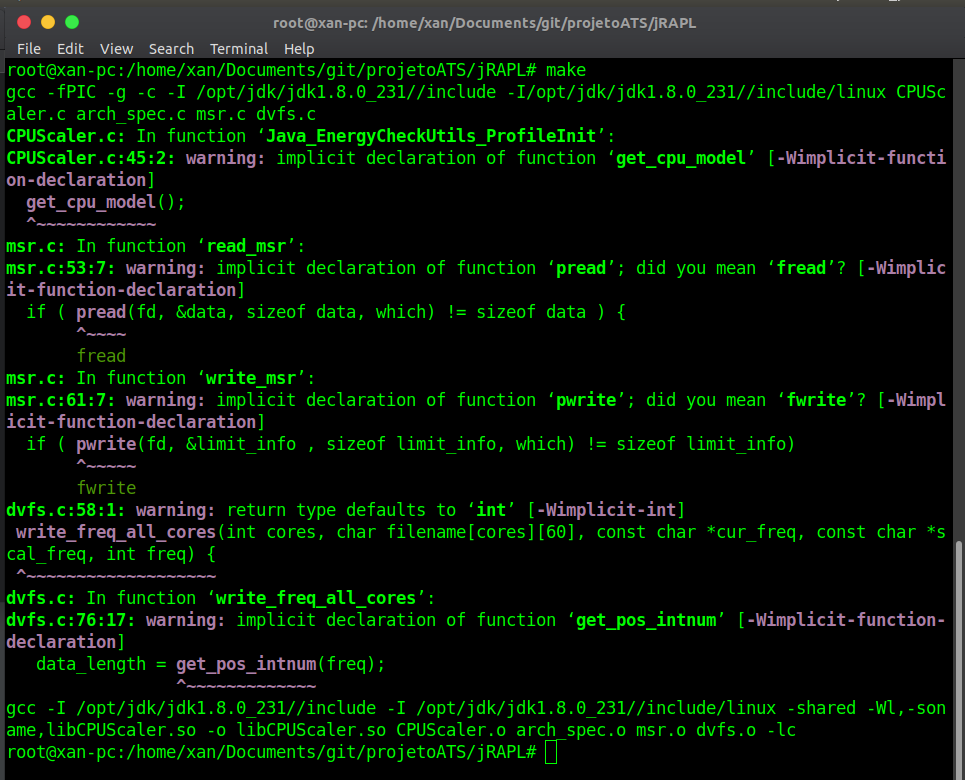
\includegraphics[scale=0.27]{images/rapl_make.png}
    \label{fig48}
    \caption{jRAPL make}
\end{figure}


Para além de executar o comando \textit{make} é necessário, no projeto, apagar o ficheiro \textit{.tmp} da respetiva pasta para que no código do \textit{try/catch} responsável por carregar a base de dados se  use o ficheiro previamente gerado \textit{generatedOutput.bak}.


\begin{figure}[H]
    \centering
    \hbox{\hspace{-4em} 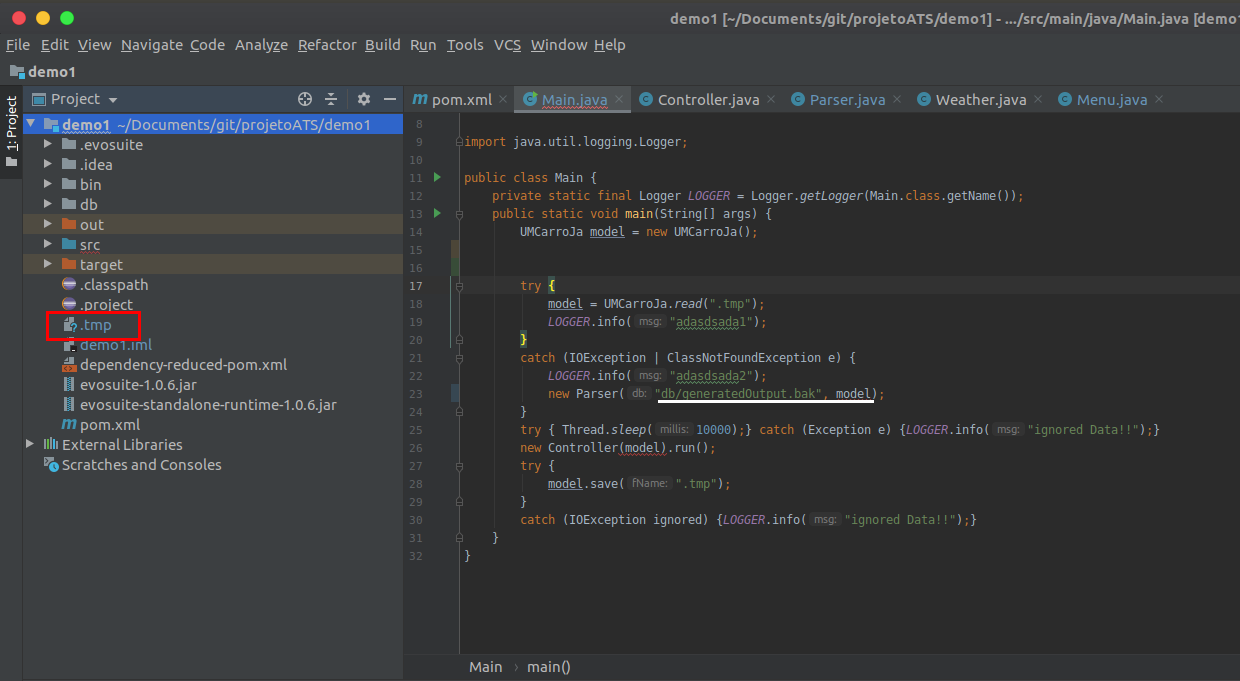
\includegraphics[width=1.2\textwidth]{images/remove_tmp.png}}
    \label{fig49}
    \caption{Remover .tmp do programa UmCarroJá}
\end{figure}

Para obter os dados de energia é necessário correr o ficheiro java do \textit{RAPL} chamado EnergyCheckUtils que é responsável por indicar o valor de energia do dram / uncore gpu energy (depende da arquitetura da cpu), do CPU e do pacote de energia.

Quando corremos pela primeira vez o java o EnergyCheckUtils deu erro de paser dos dados, por isso foi necessário efectuar uma alteração no código, ver imagem em baixo.


\begin{figure}[H]
    \hbox{\hspace{-10em} 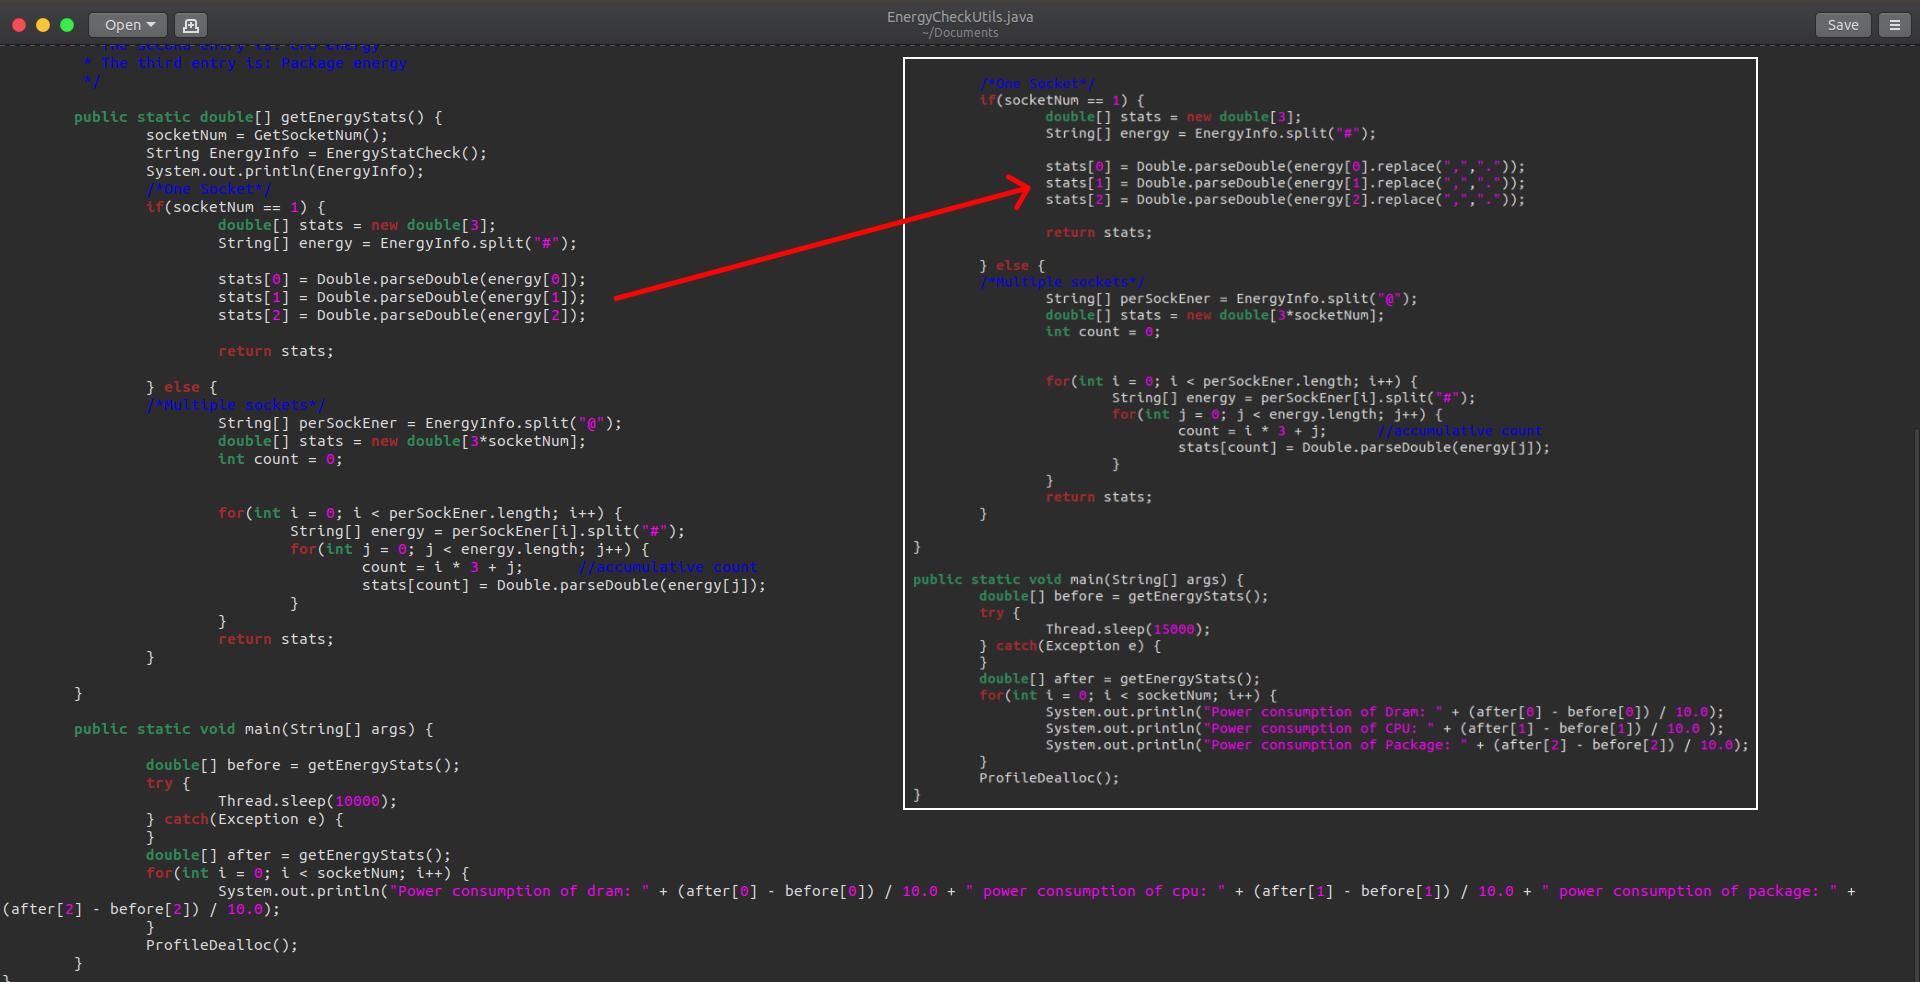
\includegraphics[width=1.5\textwidth]{images/energycheckutils.png}}
    \label{fig50}
    \caption{Alterações no ficheiro EnergyCheckUtils}
\end{figure}

Depois de corrigir o EnergyCheckUtils procedemos à execução dos comando necessário para obter os dados de energia. Comandos, \textit{sudo modprobe msr}, \textit{javac EnergyCheckUtils.java} e \textit{java EnergyCheckUtils}.

\begin{figure}[H]
    \hbox{\hspace{-8em} 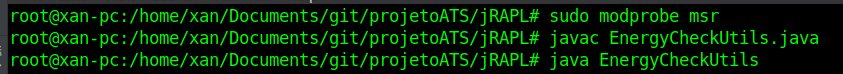
\includegraphics[width=1.5\textwidth]{images/rapl_run.png}}
    \label{fig51}
    \caption{Comandos para correr o RAPL}
\end{figure}

Para testar o UmCarroJá é primeiro necessário correr o EnergyCheckUtils e depois correr o UmCarroJá e assim obter os dados de energia tendo em consideração a solução UmCarroJá.

Efectuamos quatro testes sobre a versão final do nosso trabalho e conseguimos os seguintes resultados:
\newpage
\begin{itemize}
    \item generatedOutput5k: base de dados com 5 mil utilizadores, 5 mil proprietários, 5 mil veiculos e 10 mil avaliações 5 mil sobre os utilizadores e 5 mil sobre os proprietários;
    
        \begin{figure}[H]
            \hbox{\hspace{-8em} 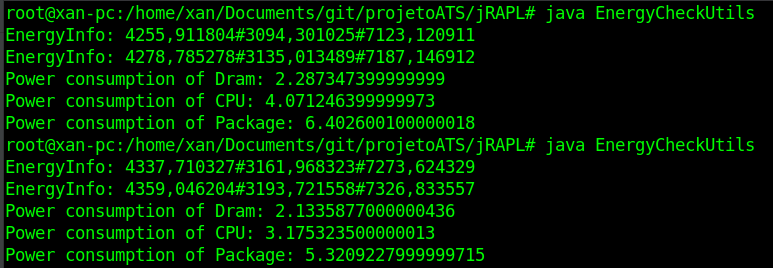
\includegraphics[width=1.5\textwidth]{images/rapl_5k.png}}
            \label{fig52}
            \caption{Testes elaborados com RAPL à solução UmCarroJá para 5k elementos}
        \end{figure}
   
    \item generatedOutput10k: base de dados com 10 mil utilizadores, 10 mil proprietários, 10 mil veiculos e 20 mil avaliações 10 mil sobre os utilizadores e 10 mil sobre os proprietários;
    
        \begin{figure}[H]
            \hbox{\hspace{-8em} 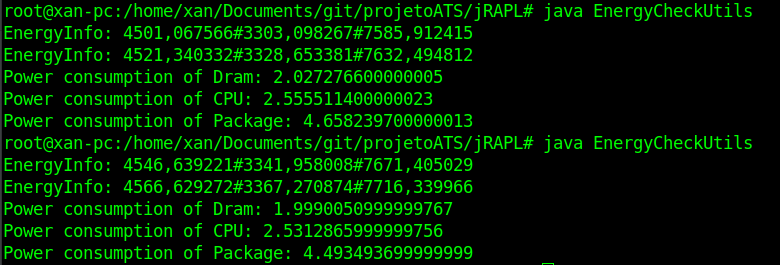
\includegraphics[width=1.5\textwidth]{images/rapl_10k.png}}
            \label{fig53}
            \caption{Testes elaborados com RAPL à solução UmCarroJá para 10k elementos}
        \end{figure}
        
    \item generatedOutput25k: base de dados com 25 mil utilizadores, 25 mil proprietários, 25 mil veiculos e 50 mil avaliações 25 mil sobre o utilizador e 25 mil sobre o proprietário;
    
        \begin{figure}[H]
            \hbox{\hspace{-8em} 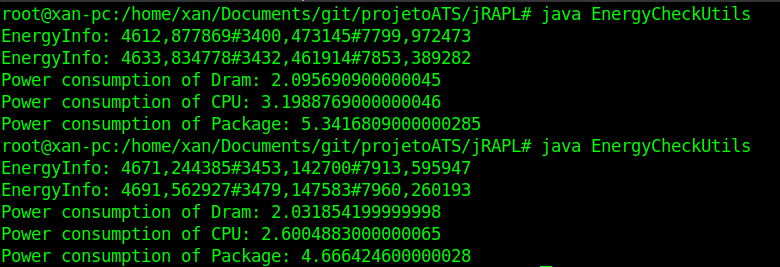
\includegraphics[width=1.5\textwidth]{images/rapl_25k.png}}
            \label{fig54}
            \caption{Testes elaborados com RAPL à solução UmCarroJá para 25k elementos}
        \end{figure}
        
    \item generatedOutput50k: base de dados com 50 mil utilizadores, 50 mil proprietários, 50 mil veiculos e 100 mil avaliações 50 mil sobre o utilizador e 50 mil sobre o proprietário;
    
        \begin{figure}[H]
            \hbox{\hspace{-8em} 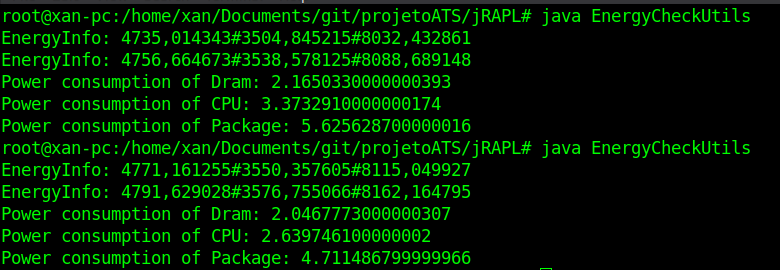
\includegraphics[width=1.5\textwidth]{images/rapl_50k.png}}
            \label{fig55}
            \caption{Testes elaborados com RAPL à solução UmCarroJá 50k elementos}
        \end{figure}
        

\end{itemize}



